\documentclass[a4paper,10pt,twocolumn]{article}
\usepackage[T1]{fontenc}
\usepackage[utf8]{inputenc}
\usepackage[icelandic]{babel}
\usepackage{graphicx}
\usepackage{subcaption}
\usepackage{hyperref}
\usepackage[inline]{enumitem}
\usepackage{biblatex} %Imports biblatex package
\addbibresource{references.bib} %Import the bibliography file
\usepackage[margin=2cm]{geometry}

\title{HiDef textíll: Tæknivædd prjónavél og þverfaglegt samstarf}
\author{Helga Ingimundardóttir}
\date{}

\begin{document}

\maketitle

\begin{abstract}
Verkefnið \emph{HiDef Textíll} sameinar hefðbundna textílvinnslu og nútímatækni með
nýsköpun í prjónavélum frá 10. áratugnum. Markmiðið er að snjallvæða úrelda prjónavél
með netsamskiptum og frjálsum hugbúnaði, sem gerir hana að öflugri lausn fyrir
skapandi notkun í dag. Verkefnið byggir á þverfaglegu samstarfi nemenda úr verkfræði,
hagnýttri stærðfræði og fatahönnun og stuðlar að aukinni þátttöku í STEAM-menntun.
Niðurstöður sýna að hægt er að nýta eldri prjónavélar á nýjan hátt og tengja íslenskan
menningararf við stafræna nýsköpun.
\end{abstract}

\section{Inngangur}
Verkefnið \emph{HiDef Textíll} á sér langa sögu og hófst sem persónulegt áhugamál 
árið 2014, þegar höfundur sá \emph{KnitterStream} \cite{knitterstream}, sem var 
listagjörningur á C2-MTL ráðstefnunni í Montréal árið 2012. Þar var gömul rafknúin 
prjónavél notuð til að umbreyta tístum á Twitter í refil. Þetta var sama vél og 
amma höfundar átti, Passap E6000 (sjá mynd \ref{fig:skema-e6000}), en hún hafði setið 
ónotuð í áraraðir. Höfundur ætlaði sér að endurtaka tilraunina og nýtti aðstöðuna 
í FabLab Reykjavík til að komast áleiðis, en verkefnið varð of tímafrekt á meðan 
höfundur var enn í doktorsnámi og í fullu starfi. Því beið það betri tíma.

Eftir umræður á kaffistofu VR-II haustið 2023, eftir að höfundur hóf störf sem 
akademískur starfsmaður, varð ljóst að hægt væri að gera þetta að rannsóknarverkefni. 
Með styrk frá \emph{Nýsköpunarsjóði námsmanna} sumarið 2024 tók verkefnið á sig nýja 
mynd, með fjölmörgum samstarfsaðilum. Prjónavélin var til húsa í vélaskála VR-III 
(sjá mynd \ref{fig:workshop}) við Hjarðarhaga 2 í Reykjavík. Nemendur höfðu einnig 
aðgang að Sprotamýri, frumkvöðlasetri HÍ í Grósku.

Verkefnið var unnið í samstarfi við Listaháskóla Íslands, frumgerðasmiðju HÍ, 
tölvunarfræðideild HÍ, rafmagns- og tölvuverkfræðideild HÍ, Textílmiðstöðina á 
Blöndósi, Heimilisiðnaðarfélagið, Þjóðminjasafn Íslands og Marel. Vélin hefur verið 
sýnd á Vísindavöku Rannís og UTmessunni hjá Ský. 

\begin{figure}
    \centering
    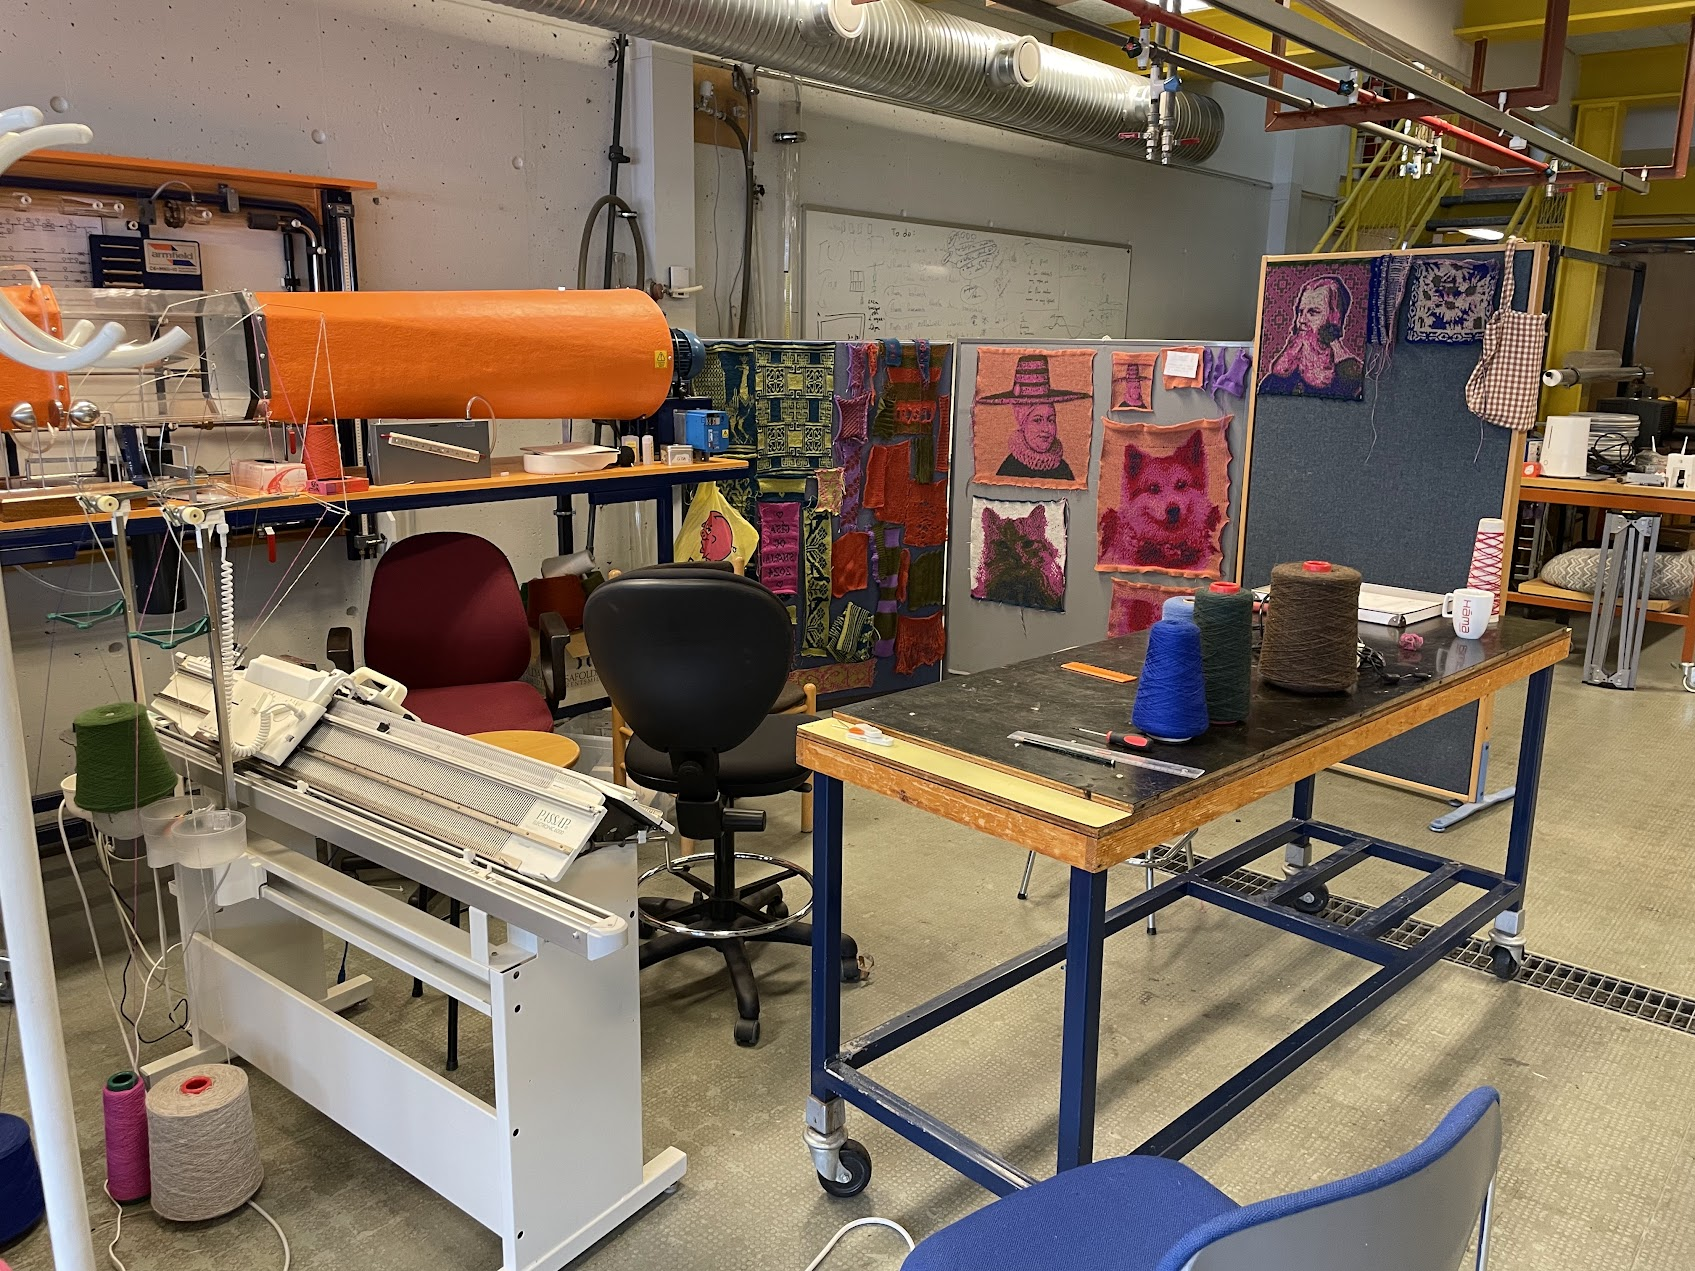
\includegraphics[width=\linewidth]{figs/workshop.jpg}
    \caption{Verkefnið var unnið í vélaskála VR-III.}
    \label{fig:workshop}
\end{figure}

\begin{figure}
    \centering
    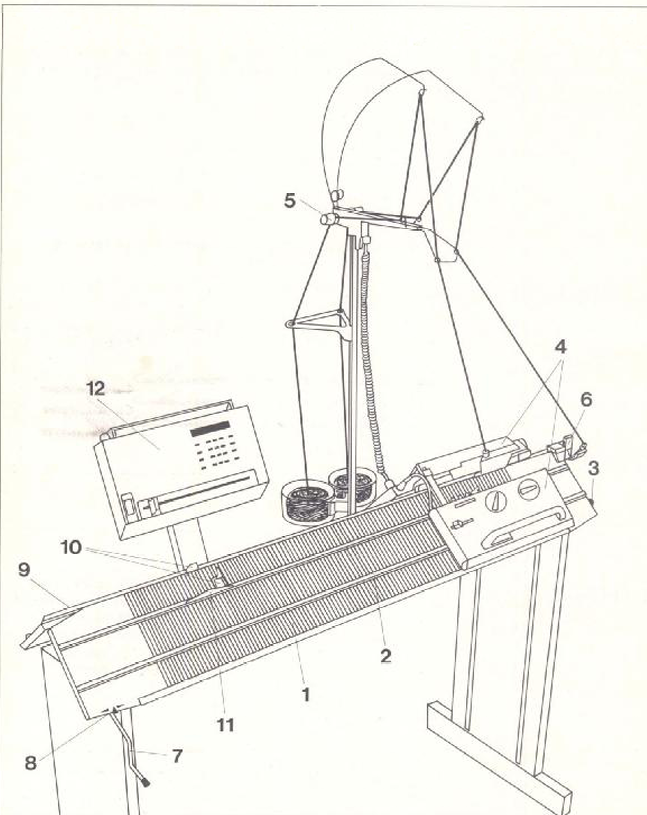
\includegraphics[width=\linewidth]{figs/skema-e6000.png}
    \caption{Skýringarmynd af Passap E6000 prjónavél.}
    \label{fig:skema-e6000}
\end{figure}

\begin{figure}
    \centering
    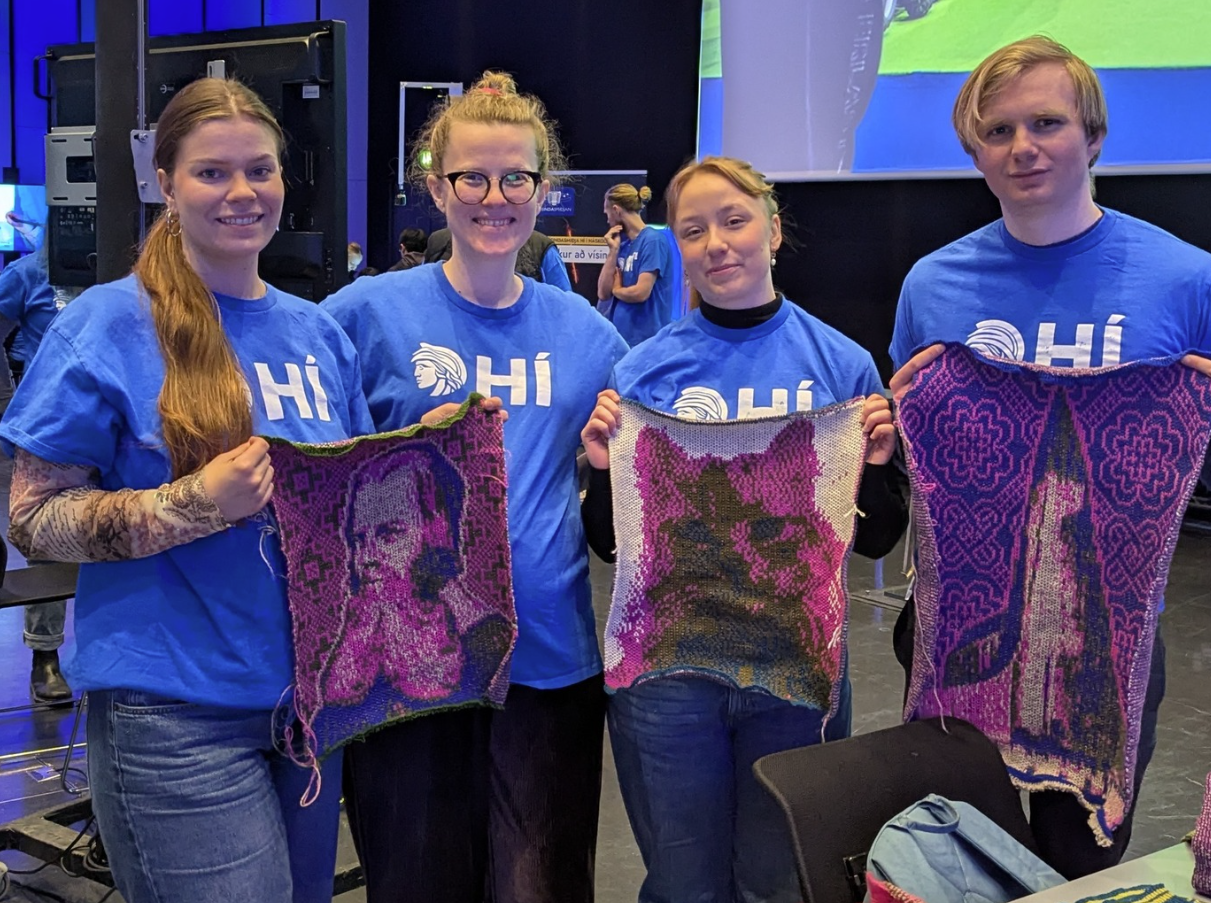
\includegraphics[width=\linewidth]{figs/hidef-team.png}
    \caption{Teymið á UTmessunni 2025: Guðrún Ísafold, Helga, Snæfríður Ebba og Elías.}
    \label{fig:team}
\end{figure}


\section{Vélrænar uppfærslur}
Til að uppfæra vélbúnað vélarinnar var upprunalega \emph{Form} tölvan (sjá hluta 12 á mynd \ref{fig:skema-e6000}) sem stýrði henni skipt út fyrir \emph{Arduino} örtölvu (sjá mynd \ref{fig:arduino}). Elías Lúðvíksson, BS nemi í vélaverkfræði við HÍ, sá um þessa uppfærslu. Eldra tölvukerfið, sem notaðist við DIN-6 snúru og lokaðan hugbúnað, var fjarlægt og í staðinn sett nýtt opið kerfi.

\begin{figure}
    \centering
    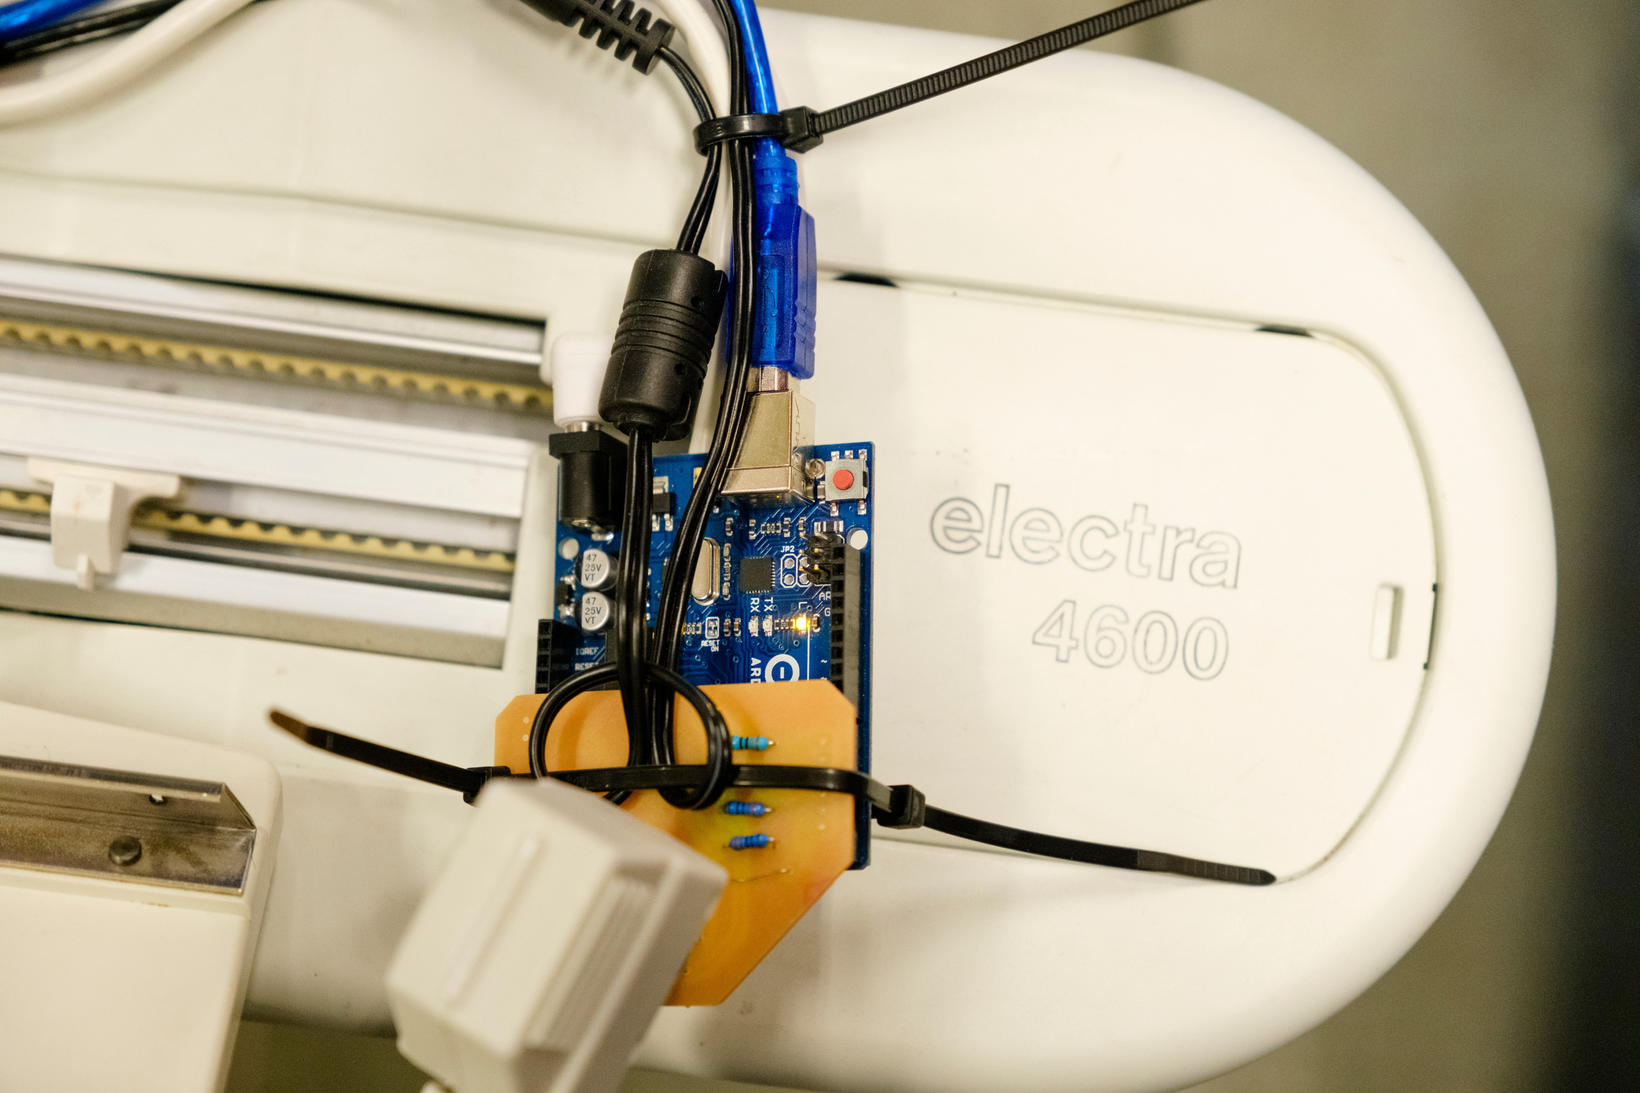
\includegraphics[width=\linewidth]{figs/arduino.jpg}
    \caption{Arduino örtölva tengd við DIN-6 tengi á Passap E6000 -- \textit{mbl.is/Kristinn Magnússon}}
    \label{fig:arduino}
\end{figure}

Vélbúnaður vélarinnar samanstendur af \begin{enumerate*}[label=(\roman*)] 
\item nálarbeði, \item sleða/lás, \item litaskiptara og \item mótor. 
\end{enumerate*} Nýja kerfið tengist sleðanum í gegnum \textit{Arduino} örtölvu, sem tekur við merkjum frá ljósaskynjurum og stýrir nálastillurum með seglum. Skynjararnir lesa göt á brautinni sem sleðinn rennur eftir og örtölvan notar þessar upplýsingar til að ákveða hvaða nálar eiga að vera virkar í hverri umferð.

Breytingarnar voru innblásnar af fyrri tilraunum hakkarýma, sérstaklega vinnu Irene Wolf og Bamberg hakksmiðju \cite{wolf, bamberg}. Nýja stýrikerfið byggir á opnum hugbúnaði og skilar sveigjanlegra kerfi fyrir sjálfvirka prjónun. 

Vélin notar tvö stýrikerfi: \begin{enumerate*}[label=(\roman*)] 
\item stýringu fyrir mótor, sem færir sleðann, og \item stýringu fyrir seglana, sem ákveða hvaða nálar eru virkar. 
\end{enumerate*} Örtölvan tekur við skipunum frá tölvu (tengt með USB snúru), sem eykur sveigjanleika og leyfir fullkomlega sjálfvirka prjónun. 

\section{Sjálfvirk mynsturgerð}
Hugbúnaðarhlutinn var þróaður til að umbreyta mynsturgögnum í prjónavænt snið.
Verkefnið byggir á vinnu Snæfríðar Ebbu Ásgeirsdóttur, BS nema í hagnýtri stærðfræði
og tölvunarfræði við HÍ, og felur í sér sjálfvirka aðlögun munstra fyrir vélina.

Litir í mynstrum eru táknaðir með heiltölum, þar sem vélin getur unnið með allt að 
fjórum litum í einu. Hver litur er prjónaður í tveimur umferðum áður en litaskipti 
eru framkvæmd. Til að tryggja samræmi í prjóninu er hver prjónlína aðskilin í 
einstakar litaraðir, þar sem hver litur er unninn sér og sendur sem aðskilin 
skipun til vélarinnar.

Með því að nýta gögn úr \emph{Íslensku Sjónabókinni} \cite{sjonabok} var skrifað 
forrit sem umbreytir útsaumsmunstrum í stafrænt prjónamynstur. Mynstur eru unnin 
með því að umbreyta háskerpumyndum í fylki af tölum, þar sem svart/hvít mynstrin 
eru einfölduð í \texttt{0} og \texttt{1}, en litaðar útfærslur nýta fjögurra litaskiptingu. Mynd \ref{fig:sjonabok_munstur} sýnir vörpunina myndrænt.

\begin{figure}
    \centering
    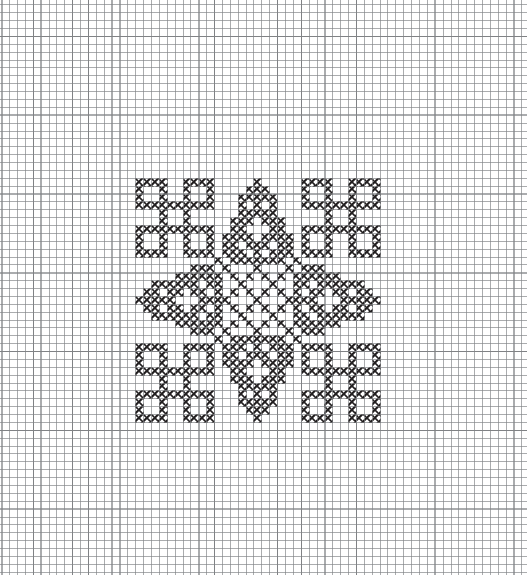
\includegraphics[width=.45\linewidth]{figs/sjonabok_before.png}
    \hfill
    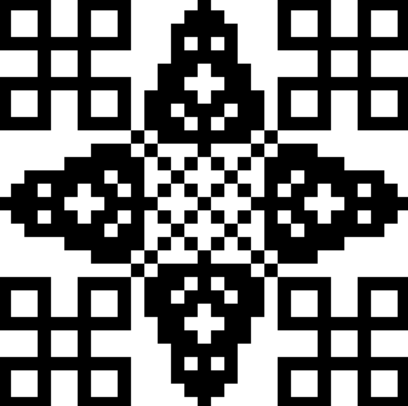
\includegraphics[width=.45\linewidth]{figs/sjonabok_after.png}
    \caption{Umbreyting munsturs úr \textit{Sjónabók} í prjónavænt snið.}
    \label{fig:sjonabok_munstur}
\end{figure}

Samhliða þessu notuðum við DALL-E spunagreindarlíkanið til að taka textalýsingu og umbreyta í mynd, sem var bætt ofan á bakgrunn úr \emph{Sjónabók} (til að viðhalda heildstæðu útliti). 
Að auki var skrifað Python-forrit sem notar \textit{Floyd-Steinberg} reikniritið 
\cite{FloydSteinberg} til að dreifa litaskiptingum og tryggja betra útlit 
mynstra á prjónuðum fleti. Með þessu ferli er hægt að umbreyta flóknum 
myndum í prjónamynstur sem vélin getur útfært á nákvæman hátt, einsog sjá má í mynd \ref{fig:hallgrimskirkja} af Hallgrímskirkju.

\begin{figure}
    \centering
    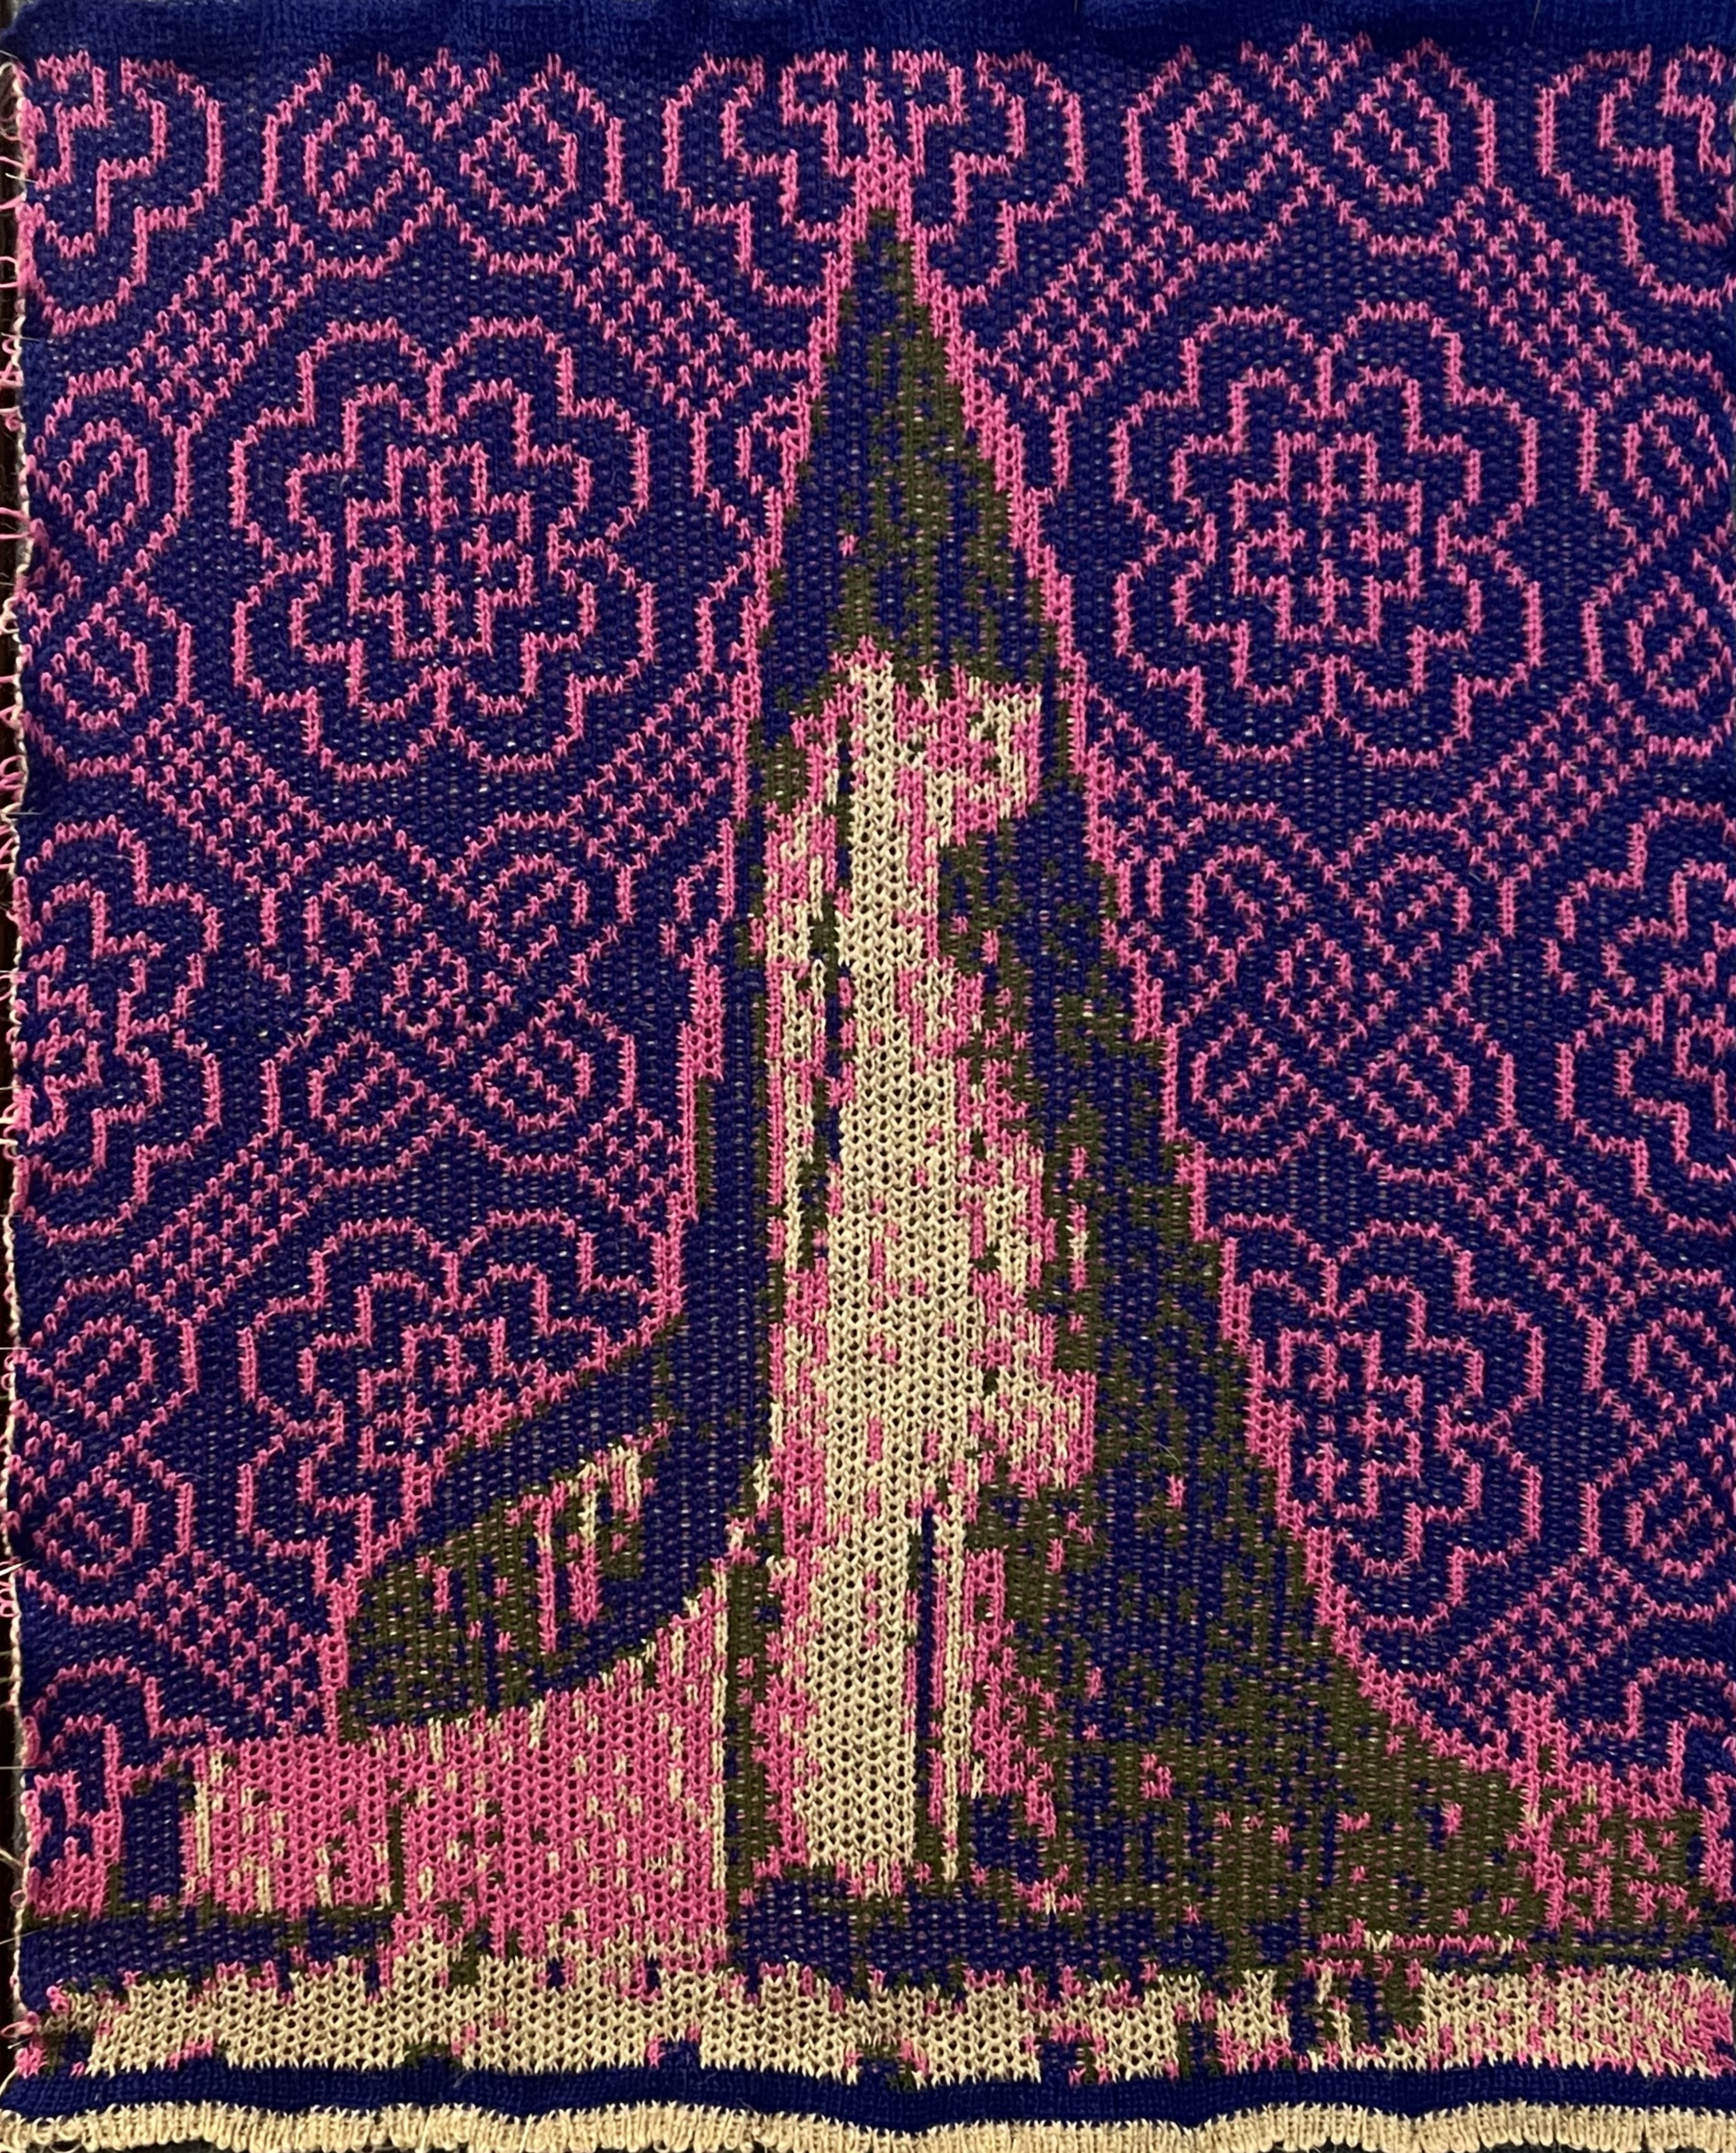
\includegraphics[width=\linewidth]{figs/hallgrimskirkja.JPG}
    \caption{Hallgrímskirkja með bakgrunni úr \emph{Sjónabók}}
    \label{fig:hallgrimskirkja}
\end{figure}


\section{Prjón og hönnunarvinna}
Fatahönnunin, sem Guðrún Ísafold Hilmarsdóttir, BA nemi í fatahönnun við LHÍ, sá um, var órjúfanlegur hluti af verkefninu. Hún veitti fagurfræðilega leiðsögn og lagði áherslu á hvernig útfærsla á mynstrum tengdist takmörkunum og möguleikum vélarinnar.

Ferlið var byggt á Design Thinking \cite{designthinking} aðferðafræðinni og þróaðist í gegnum stöðugar tilraunir og endurbætur. Í fyrstu var lögð áhersla á einföld tvílita mynstur og grunnprufur til að skilja hvernig vélbúnaðurinn tók við nýjum fyrirmælum. Með aukinni reynslu tókst að bæta við þriðja og síðar fjórða litnum, en það krafðist breytinga á prjónatækninni sjálfri.

Fyrstu prufurnar (sjá myndir \ref{fig:hallo_heimur}, \ref{fig:repeat} og \ref{fig:flower}) leiddu í ljós að fyrri vélrænar breytingar höfðu áhrif á gæði prjónsins. Með náinni samvinnu við Elías og Snæfríði voru þessir vankantar greindir og aðlagaðir jafnóðum í kóðun og vélrænum útfærslum. Guðrún lagði áherslu á að hönnunin tæki mið af þessum takmörkunum og vann með þær fremur en á móti þeim.

Til að nýta þegar unnar prjónaprufur var fatnaður hannaður út frá mynstrunum, með áherslu
á sjálfbærni og samræmda hönnunarheild. Þessi nálgun birtist skýrt í fatnaðarútfærslunum 
á mynd \ref{fig:designproposal}.

\begin{figure}
    \centering
    \begin{subfigure}[b]{\linewidth}
        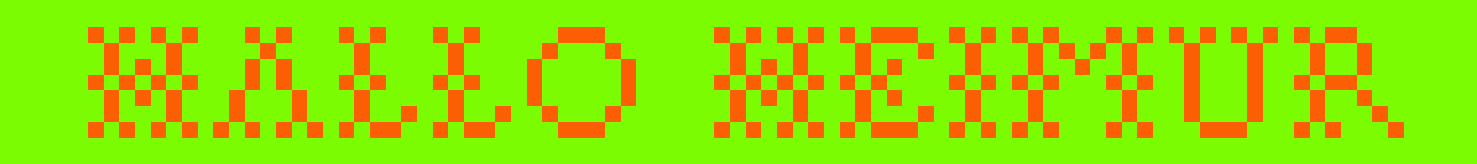
\includegraphics[width=\linewidth, clip=true, trim=0 5mm 0 0]{figs/hallo_heimur_forskrift.png}
        \caption{Forskrift}
    \end{subfigure}
    \\
    \begin{subfigure}[b]{0.48\linewidth}
        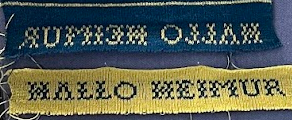
\includegraphics[width=\linewidth, clip=true, trim=0 5mm 0 0]{figs/hallo_heimur_prjon.png}
        \caption{Fyrsta atrenna}
    \end{subfigure}
    \hfill
    \begin{subfigure}[b]{0.48\linewidth}
        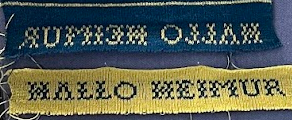
\includegraphics[width=\linewidth, clip=true, trim=0 0 0 5mm]{figs/hallo_heimur_prjon.png}
        \caption{Seinni atrenna}
    \end{subfigure}
    \caption{Þróun á prjónamynstri fyrir \textit{Halló heimur}.}
    \label{fig:hallo_heimur}
\end{figure}


\begin{figure}
    \centering
    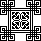
\includegraphics[width=0.45\linewidth]{figs/thjms5898_268.png}
    \hfill
    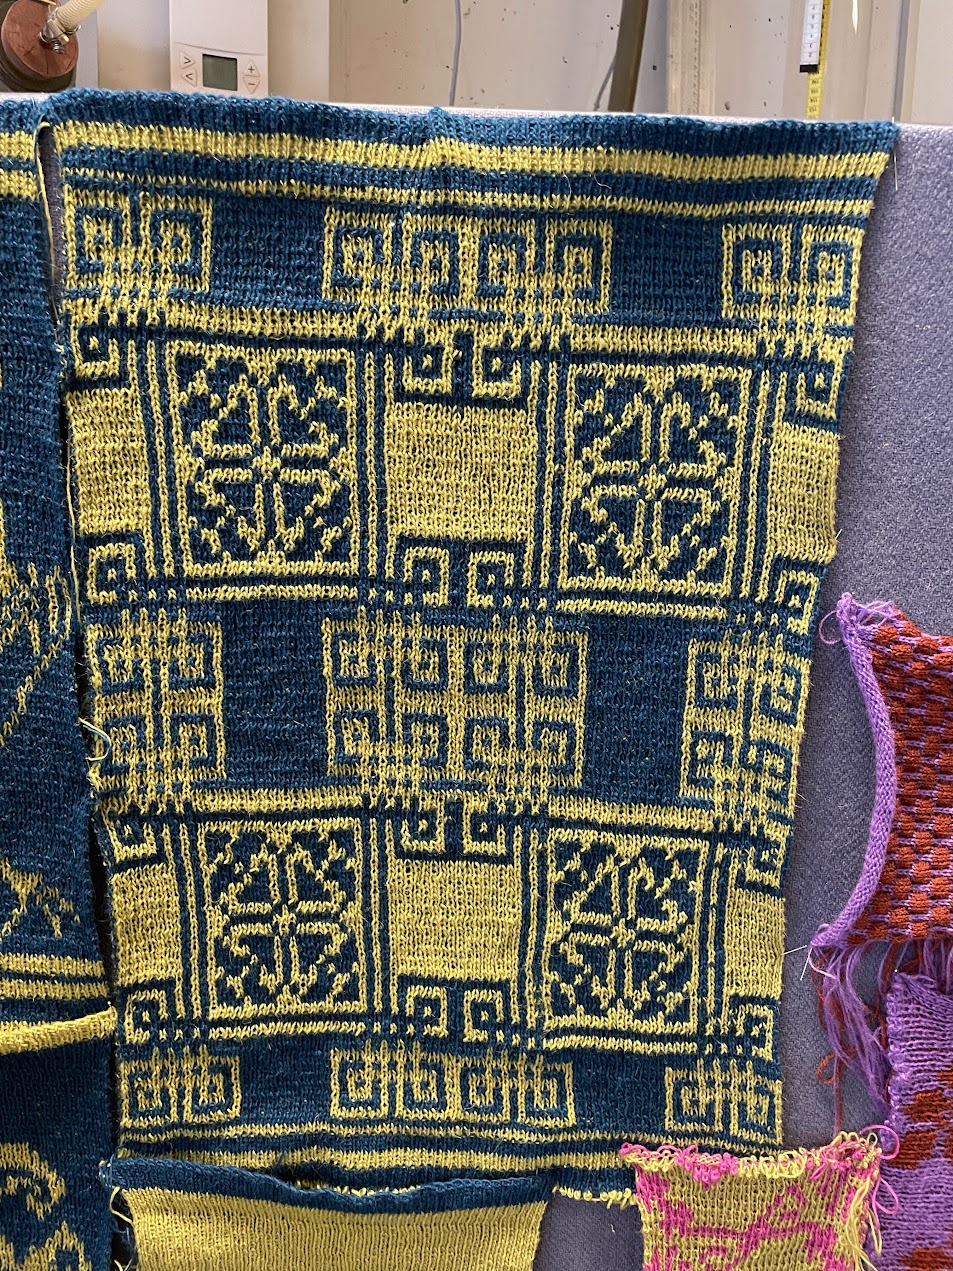
\includegraphics[width=0.45\linewidth]{figs/repeat.jpg}
    \caption{Endurtekið mótif, bls. 268 í \textit{Sjónabók} (Þjms. 5898)}
    \label{fig:repeat}
\end{figure}

\begin{figure}
    \centering
    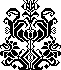
\includegraphics[width=0.45\linewidth]{figs/thjms5898_210.png}
    \hfill
    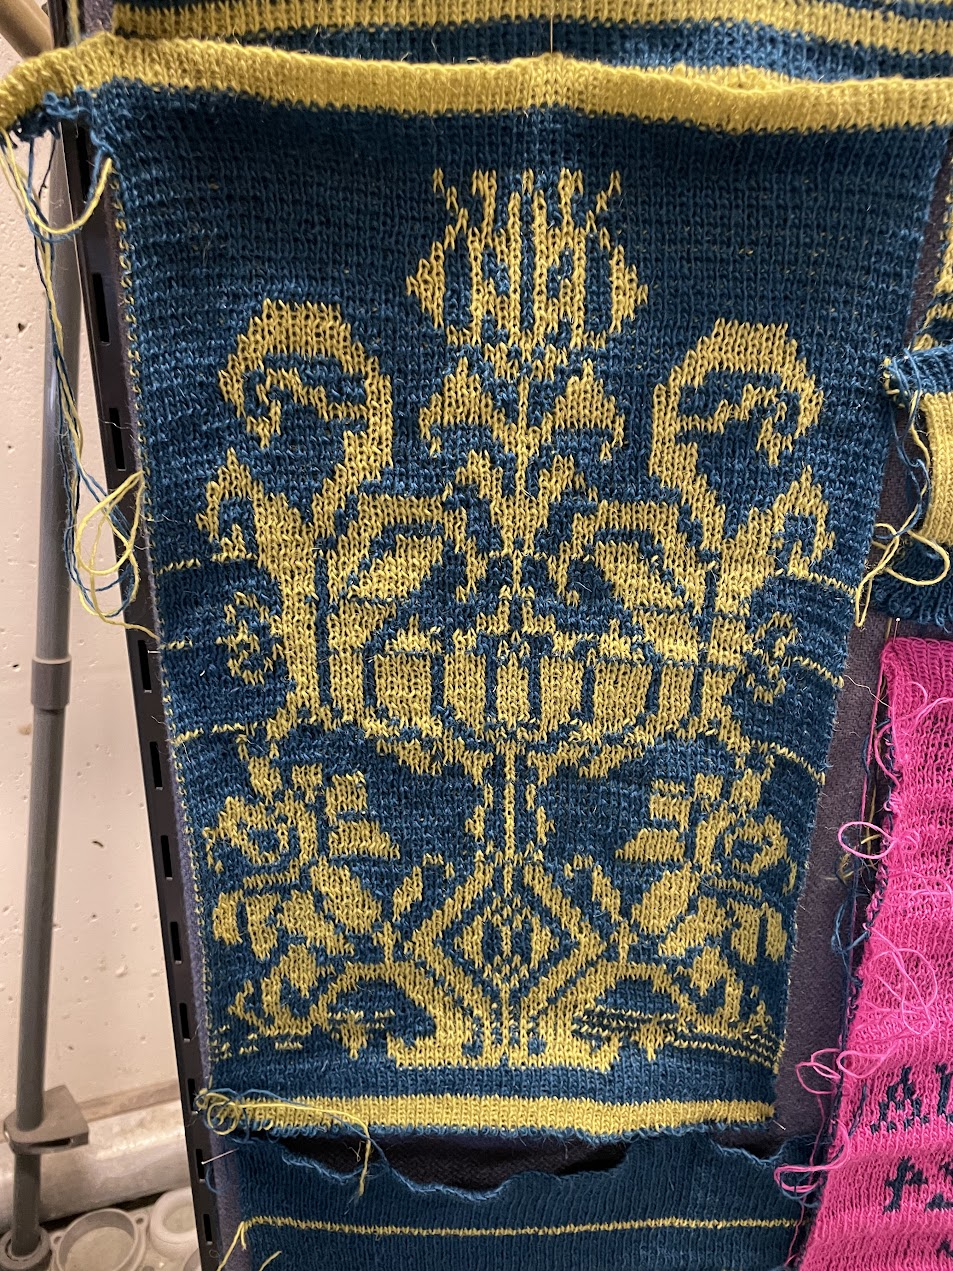
\includegraphics[width=0.45\linewidth]{figs/flower.jpg}
    \caption{Blóm, bls. 210 í \textit{Sjónabók} (Þjms. 5898)}
    \label{fig:flower}
\end{figure}

\begin{figure}
    \centering
    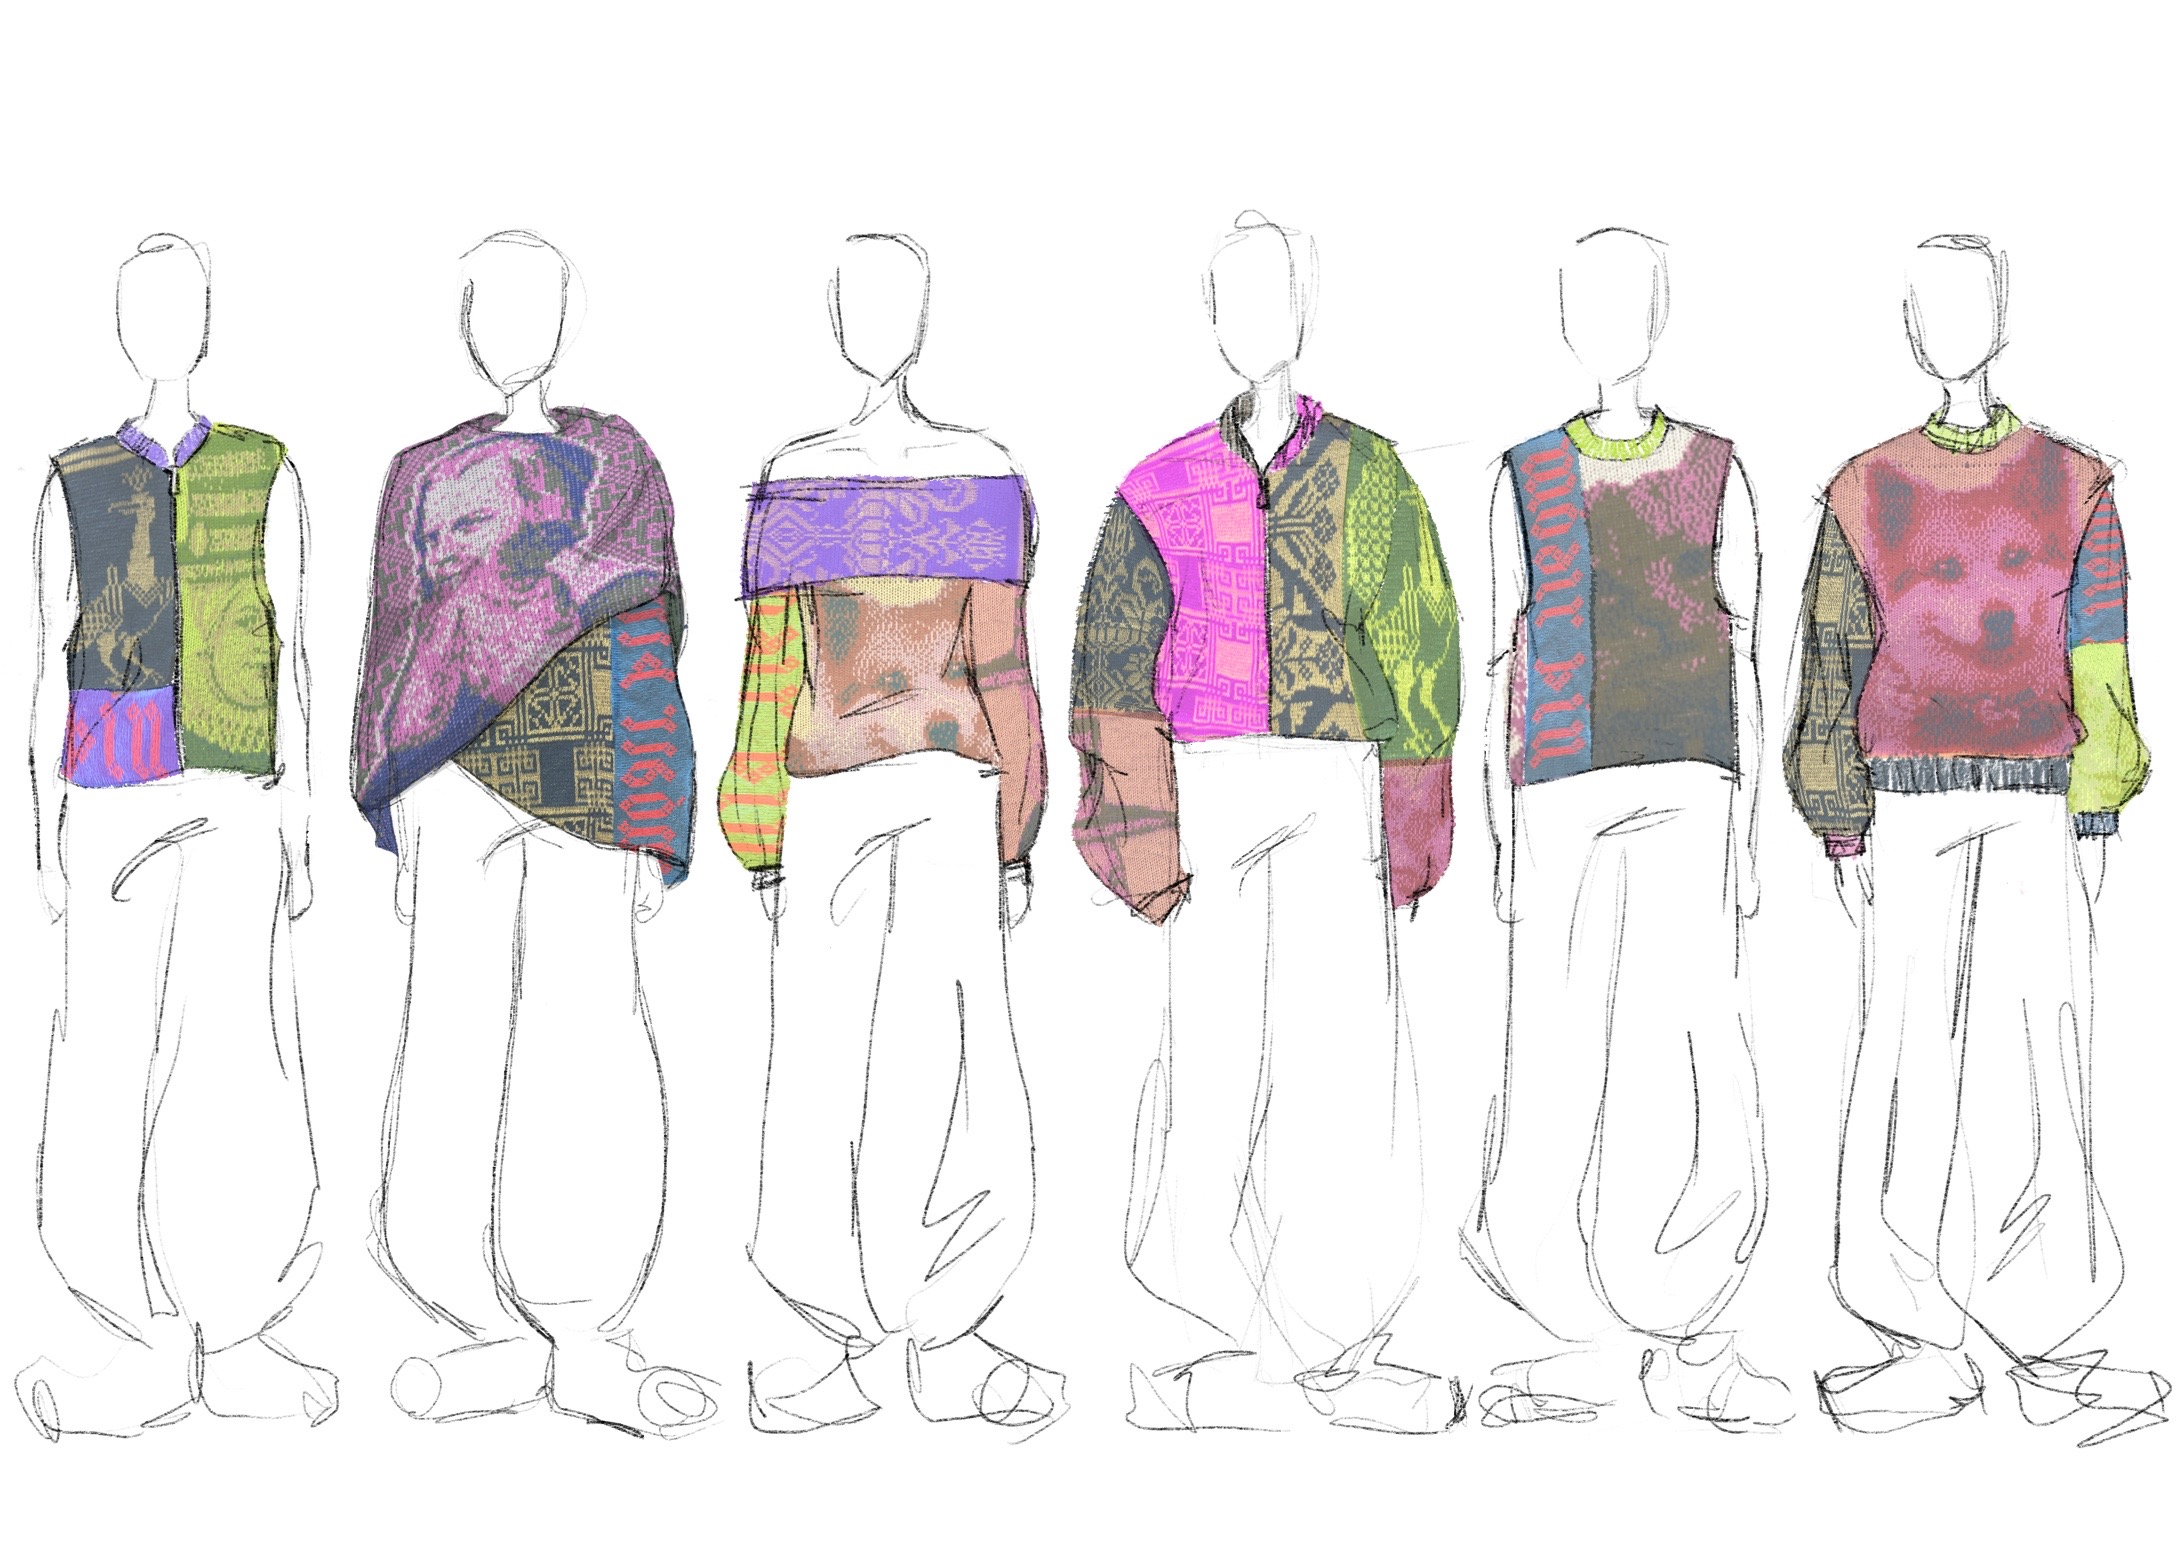
\includegraphics[width=\linewidth]{figs/collection.JPG}
    \caption{Útfærslur á fatnaði út frá prjónaprufum verkefnisins.}
    \label{fig:designproposal}
\end{figure}


\section{Þverfaglegt samstarf}
Verkefnið sýnir hvernig samvinna milli ólíkra fræðasviða getur skapað afurð sem er stærri en hver einstakur þátttakandi. Samstarf Guðrúnar (hönnun), Snæfríðar (hugbúnaður) og Elíasar (vélbúnaður) tryggði að verkefnið varð heildstætt, þar sem allir þættir tengdust í einni samþættri lausn.

Fyrstu prufurnar voru sérstaklega mikilvægur hluti ferlisins, þar sem þær afhjúpuðu bæði styrkleika og veikleika breytinganna á vélinni. Ef breyting á vélbúnaði eða hugbúnaði skilaði sér ekki rétt í prjóninu, þurfti að endurgreina ferlið og finna út hvað olli vandanum. Þetta gerði það að verkum að teymið lærði ekki bara á sín sérsvið heldur einnig á hvernig þau tengdust.

Án þessa samstarfs hefði hvorugt -- hvorki véla- og hugbúnaðarkerfið né fatahönnunin -- getað náð því fulla möguleikasviði sem verkefnið endaði með.


\section{Framtíðarhorfur og næstu skref}
Næsta markmið verkefnisins er að gera vélina auðveldari til flutnings fyrir viðburði og bæta sjálfvirkni í litastýringu. 
Stefnt er að því að þróa áfram notendavænt vefviðmót sem gerir gestum og gangandi kleift að senda inn mynstur og prjóna þau í rauntíma þegar vélin er til sýnis.

Einnig er áhersla lögð á áframhaldandi samþættingu stafrænnar listsköpunar við handverk, 
þar sem prjónaferlið er nýtt sem skapandi miðill. Með þróun sjálfvirkrar mynsturgerðar og aðlögunar að sögulegum mynstrum 
er unnið að því að tengja saman forna handverkshefð og nútímatækni.

Stefnt er að sýningu á \emph{Hönnunarmars 2026}, þar sem afrakstur verkefnisins verður kynntur. Með því verður sýnt hvernig
samspil hugbúnaðar, vélbúnaðar og hönnunar getur leitt til nýrra möguleika í sjálfbærri textílframleiðslu.

Öll þróun verkefnisins er opin og aðgengileg í gegnum GitHub, \url{https://github.com/hideftextiles/}, þar sem hægt er að fylgjast með þróun hugbúnaðarins og nota hann í eigin verkefnum. 

\printbibliography

\end{document}
